\documentclass[12pt]{article}
\usepackage{amsmath, amssymb}
\usepackage{booktabs}
\usepackage{geometry}
\usepackage{pgfplots}
\pgfplotsset{compat=1.18}
\usepackage{xcolor}
\geometry{margin=1in}

\title{Data Generating Mechanism for the Three-Time-Point SNTTEM Simulation}
\date{}

\begin{document}
\maketitle

\section{Overview}

We simulate longitudinal data for $n$ individuals over three time points
$t \in \{0, 1, 2\}$.  At each time point we observe a covariate $L_t$, an
eligibility indicator $I_t$, and a binary treatment $A_t \in \{0,1\}$.  A
single binary outcome $Y$ is measured at the end of follow-up.  The data
are generated sequentially in the temporal order
$I_0, L_0, A_0 \;\to\; I_1, L_1, A_1 \;\to\; I_2, L_2, A_2 \;\to\; Y$.

The simulation has five scalar parameters:
\begin{itemize}
  \item $\psi_{03}, \psi_{13}, \psi_{23}$: blip parameters encoding the
        causal effect of treatment at each time point on $\log P(Y=1)$;
  \item $p_I \in (0,1)$: marginal probability of eligibility at times 1
        and 2 (default $p_I = 0.5$);
  \item $p_h \in (0,1)$: probability that treatment is \emph{held} (i.e.\
        unchanged) from one period to the next (default $p_h = 0.05$).
\end{itemize}

\section{Time $t = 0$}

\paragraph{Eligibility.}
Every individual is eligible at baseline:
\[
  I_0 = 1.
\]

\paragraph{Baseline covariate.}
\[
  L_0 \sim \mathrm{Uniform}(0,\, 0.5).
\]

\paragraph{Baseline treatment.}
\[
  A_0 \mid L_0 \sim \mathrm{Bernoulli}\!\left(\mathrm{expit}(-1 + L_0)\right),
  \qquad \mathrm{expit}(x) = \frac{e^x}{1+e^x}.
\]

\section{Time $t = 1$}

\paragraph{Eligibility.}
\[
  I_1 \sim \mathrm{Bernoulli}(p_I), \quad \text{independent of all other variables.}
\]

\paragraph{Covariate.}
$L_1$ depends on the preceding treatment $A_0$ via a clipped normal:
\[
  L_1^* \mid A_0 \sim \mathcal{N}(-0.5\, A_0,\; 1),
  \qquad
  L_1 = \mathrm{clip}(L_1^*;\; -1.5,\; -0.5).
\]

\paragraph{Treatment.}
Treatment at time 1 is generated by a \emph{random switching} mechanism: with
probability $p_h$ the treatment is held at its previous value, and with
probability $1-p_h$ it switches:
\[
  A_1 \mid A_0 =
  \begin{cases}
    A_0     & \text{with probability } p_h, \\
    1 - A_0 & \text{with probability } 1 - p_h.
  \end{cases}
\]

\section{Time $t = 2$}

\paragraph{Eligibility.}
\[
  I_2 \sim \mathrm{Bernoulli}(p_I), \quad \text{independent of all other variables.}
\]

\paragraph{Covariate.}
\[
  L_2^* \mid A_1 \sim \mathcal{N}(-0.5\, A_1,\; 1),
  \qquad
  L_2 = \mathrm{clip}(L_2^*;\; -1.5,\; -0.5).
\]

\paragraph{Treatment.}
\[
  A_2 \mid A_1 =
  \begin{cases}
    A_1     & \text{with probability } p_h, \\
    1 - A_1 & \text{with probability } 1 - p_h.
  \end{cases}
\]

\section{Outcome}

The binary outcome $Y$ follows a log-linear model:
\[
  Y \mid \bar{A}, \bar{L}, \bar{I}
  \;\sim\;
  \mathrm{Bernoulli}\!\left(\exp(\eta)\right),
\]
where the log-risk $\eta$ is
\begin{align}
  \eta \;=\; {}&
  -1.5
  \;+\; \psi_{03}\, L_0\, A_0 \notag \\
  &+\; I_1\, \psi_{13}\,(1 + L_1)\,(A_1 - A_0)
   \;+\; (1-I_1)\, \psi_{13}\, \tfrac{L_1}{3}\,(A_1 - A_0) \notag \\
  &+\; I_2\, \psi_{23}\,(1 + L_2)\,(A_2 - A_1)
   \;+\; (1-I_2)\, \psi_{23}\, \tfrac{L_2}{3}\,(A_2 - A_1). \label{eq:logp}
\end{align}

\section{Structural Blip Functions}

The log-risk in~\eqref{eq:logp} is constructed from \emph{blip functions}
$\gamma_t$, which represent the causal effect on $\log P(Y=1)$ of
incrementing treatment at time $t$ by one unit, conditional on the
observed history.  The blip functions are:
\begin{align}
  \gamma_{03}(L_0;\, \psi_{03}) &= \psi_{03}\, L_0, \\
  \gamma_{13}(L_1;\, \psi_{13}) &= \psi_{13}\,(1 + L_1), \\
  \gamma_{23}(L_2;\, \psi_{23}) &= \psi_{23}\,(1 + L_2).
\end{align}
For an \emph{eligible} individual ($I_t = 1$) the blip function is
$\gamma_t(\cdot)$ evaluated at the observed $L_t$, while for an
\emph{ineligible} individual ($I_t = 0$) the blip is attenuated by a
factor of $L_t/3\,(1+L_t)^{-1}$ relative to the eligible case, reflecting a
reduced treatment effect in ineligible strata.

\section{Summary Table}

\begin{center}
\begin{tabular}{lll}
\toprule
Variable & Distribution & Parameters \\
\midrule
$I_0$    & Degenerate at 1 & --- \\
$L_0$    & $\mathrm{Uniform}(0, 0.5)$ & --- \\
$A_0$    & $\mathrm{Bernoulli}(\mathrm{expit}(-1+L_0))$ & $L_0$ \\
$I_1$    & $\mathrm{Bernoulli}(p_I)$ & $p_I$ \\
$L_1$    & $\mathrm{clip}(\mathcal{N}(-0.5A_0,1),\,-1.5,\,-0.5)$ & $A_0$ \\
$A_1$    & Switch from $A_0$ with prob $1-p_h$ & $p_h$, $A_0$ \\
$I_2$    & $\mathrm{Bernoulli}(p_I)$ & $p_I$ \\
$L_2$    & $\mathrm{clip}(\mathcal{N}(-0.5A_1,1),\,-1.5,\,-0.5)$ & $A_1$ \\
$A_2$    & Switch from $A_1$ with prob $1-p_h$ & $p_h$, $A_1$ \\
$Y$      & $\mathrm{Bernoulli}(\exp(\eta))$ & see \eqref{eq:logp} \\
\bottomrule
\end{tabular}
\end{center}

\section{Simulation Results: Empirical Variance of $\hat\psi_{23}$ (Three-Step Estimator)}

Figure~\ref{fig:var_psi23} shows the empirical variance of the three-step
estimator of $\psi_{23}$ as a function of the treatment-hold probability
$p_h \in \{0.4, 0.6, 0.8\}$, separately for each eligibility proportion
$p_I \in \{0.25, 0.50, 0.75, 1.00\}$.  True parameter values are
$\psi_{03} = \psi_{13} = \psi_{23} = 1$.

Two patterns are consistent across all $p_I$ levels.  First, variance
decreases monotonically as $p_I$ increases: greater eligibility provides
more variation in blip contrasts $(A_t - A_{t-1})$, which tightens the
estimating equations for $\psi_{23}$.  Second, the relationship between
$p_h$ and variance is non-monotone: variance is lowest at an intermediate
hold probability ($p_h = 0.6$ for $p_I \geq 0.5$, $p_h = 0.4$ for
$p_I = 0.25$) and rises again at $p_h = 0.8$.  At high $p_h$ treatments
rarely change, so the contrast $A_2 - A_1$ has low variation and the
estimator for the time-2 blip $\gamma_{23}$ becomes poorly identified.

\begin{figure}[ht]
\centering
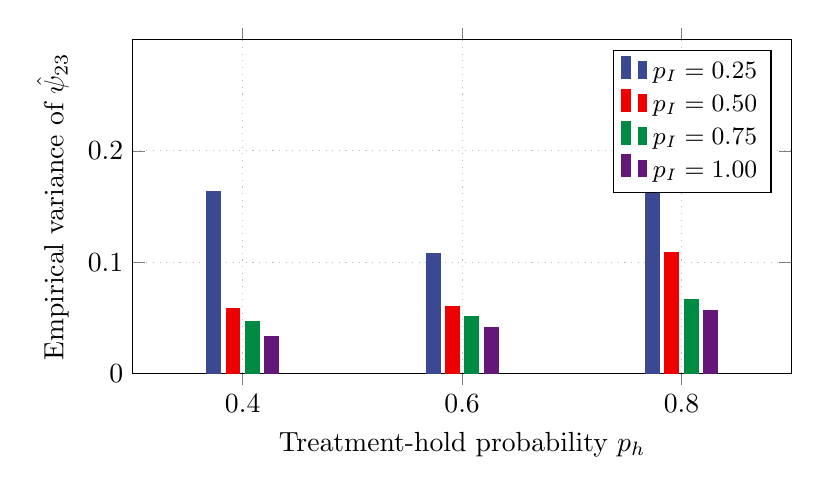
\begin{tikzpicture}
\begin{axis}[
  ybar,
  bar width=5pt,
  width=0.82\textwidth,
  height=0.48\textwidth,
  xlabel={Treatment-hold probability $p_h$},
  ylabel={Empirical variance of $\hat\psi_{23}$},
  symbolic x coords={0.4, 0.6, 0.8},
  xtick=data,
  enlarge x limits=0.25,
  legend style={at={(0.97,0.97)}, anchor=north east, font=\small},
  grid=major,
  grid style={dotted, gray!50},
  ymin=0,
]
% p_I = 0.25
\addplot[fill={rgb,255:red,59;green,73;blue,146}, draw={rgb,255:red,59;green,73;blue,146}]
  coordinates {(0.4, 0.163589) (0.6, 0.107768) (0.8, 0.272594)};
\addlegendentry{$p_I = 0.25$}

% p_I = 0.50
\addplot[fill={rgb,255:red,238;green,0;blue,0}, draw={rgb,255:red,238;green,0;blue,0}]
  coordinates {(0.4, 0.058323) (0.6, 0.060597) (0.8, 0.108974)};
\addlegendentry{$p_I = 0.50$}

% p_I = 0.75
\addplot[fill={rgb,255:red,0;green,139;blue,69}, draw={rgb,255:red,0;green,139;blue,69}]
  coordinates {(0.4, 0.046525) (0.6, 0.051144) (0.8, 0.066644)};
\addlegendentry{$p_I = 0.75$}

% p_I = 1.00
\addplot[fill={rgb,255:red,99;green,24;blue,121}, draw={rgb,255:red,99;green,24;blue,121}]
  coordinates {(0.4, 0.033320) (0.6, 0.041396) (0.8, 0.056317)};
\addlegendentry{$p_I = 1.00$}
\end{axis}
\end{tikzpicture}
\caption{Empirical variance of the three-step estimator $\hat\psi_{23}$
  by treatment-hold probability $p_h$, stratified by eligibility proportion
  $p_I$.  Each bar is computed over Monte Carlo replications with
  $\psi_{03}=\psi_{13}=\psi_{23}=1$.}
\label{fig:var_psi23}
\end{figure}

The numerical values underlying Figure~\ref{fig:var_psi23} are reproduced
in Table~\ref{tab:var_psi23}.

\begin{table}[ht]
\centering
\caption{Empirical variance of $\hat\psi_{23}$, three-step estimator.}
\label{tab:var_psi23}
\begin{tabular}{cccc}
\toprule
$p_I$ & $p_h = 0.4$ & $p_h = 0.6$ & $p_h = 0.8$ \\
\midrule
0.25 & 0.1636 & 0.1078 & 0.2726 \\
0.50 & 0.0583 & 0.0606 & 0.1090 \\
0.75 & 0.0465 & 0.0511 & 0.0666 \\
1.00 & 0.0333 & 0.0414 & 0.0563 \\
\bottomrule
\end{tabular}
\end{table}

\end{document}
